\part{linux 基础知识}

在第一部门中先了解linux基础操作知识,他们包括系统知识,网络知识,


\chapter{系统基础}

\section{centos7 安装}

CentOS 7 网卡名不以eth0开始原因,是由于systemd 和 udev 引入了一种新的网络设备命名方式–一致网络设备命名(CONSISTENT NETWORK DEVICE NAMING) 。可以根据固件、拓扑、位置信息来设置固定名字,带来的好处是命名自动化,名字完全可预测,在硬件坏了以后更换也不会影响设备的命名,这样可以让硬件的更换无缝化。带来的不利是新的设备名称比传统的名称难以阅读。比如心得名称是enp5s0.

想要改为像centos6一样以eth0开始的名称有两种方法,在出现安装新系统的时候按下tab键,在kernel启动选项中增加 net.ifnames=0 biosdevname=0 


\begin{figure}[!ht]
    \centering    
     \caption{\label{Fig:async} Asynchronous I/O model}
    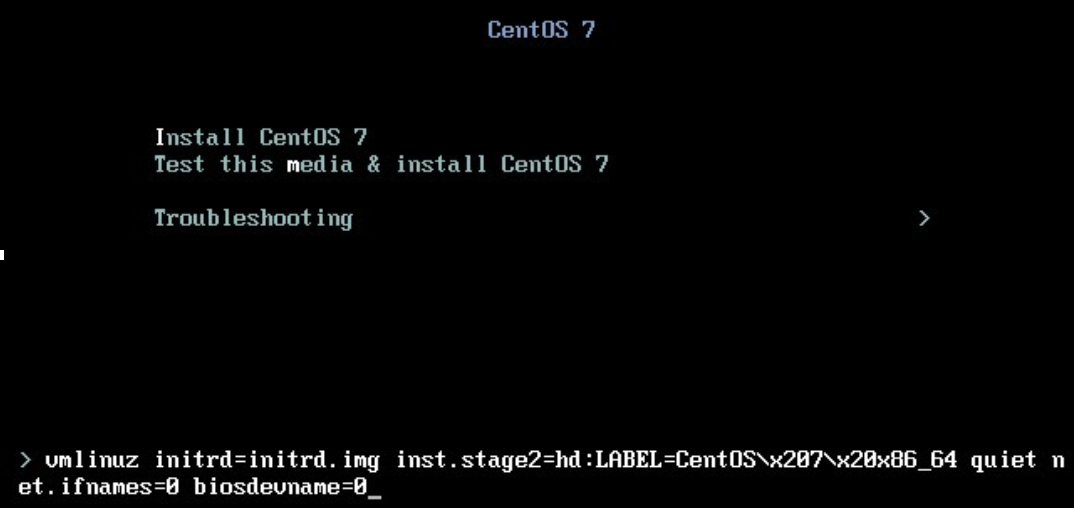
\includegraphics[width=0.8\textwidth]{./images/centos-bios.png}  
\end{figure}

当然,如果在安装时忘记操作了也可以在启动后操作。在 /etc/sysconfig/grub下相应位置加上这两个参数,然后再改网卡名既可

\begin{lstlisting}
GRUB_CMDLINE_LINUX=”rd.lvm.lv=vg0/swap vconsole.keymap=us crashkernel=auto  vconsole.font=latarcyrheb-sun16 net.ifnames=0 biosdevname=0 rd.lvm.lv=vg0/usr rhgb quiet”

grub2-mkconfig -o /boot/grub2/grub.cfg

\end{lstlisting}

安装完系统后一般需要关闭selinux, NetworkManager, firewalld, 需要安装net-tools, lsof, tcpdump, epel,

\subsection{桥接}

一、网卡桥接设置:

1、网卡配置文件:

[root@localhost /]# vim /etc/sysconfig/network-scripts/ifcfg-enp8s0

TYPE=Ethernet
DEVICE=enp8s0
NAME=enp8s0
BOOTPROTO=none
ONBOOT=yes
BRIDGE=br0

 2、网桥配置文件:

[root@localhost /]# vim /etc/sysconfig/network-scripts/ifcfg-br0

TYPE=Bridge
DEVICE=br0
BOOTPROTO=static
ONBOOT=yes
IPADDR=192.168.1.200
NETMASK=255.255.255.0
GATEWAY=192.168.1.1
DNS1=114.114.114.114


二、网卡绑定设置:

1、网卡配置文件01:

[root@localhost /]# vim /etc/sysconfig/network-scripts/ifcfg-enp6s0f0

TYPE=Ethernet
DEVICE=enp6s0f0
NAME=enp6s0f0
BOOTPROTO=none
ONBOOT=yes
USERCTL=no
MASTER=bond0
SLAVE=yes
2、网卡配置文件02:

[root@localhost /]# vim /etc/sysconfig/network-scripts/ifcfg-enp6s0f1

TYPE=Ethernet
DEVICE=enp6s0f1
NAME=enp6s0f1
BOOTPROTO=none
ONBOOT=yes
USERCTL=no
MASTER=bond0
SLAVE=yes
3、网桥配置文件:

[root@localhost /]# vim /etc/sysconfig/network-scripts/ifcfg-bond0

TYPE=Ethernet
DEVICE=bond0
BOOTPROTO=static
ONBOOT=yes
USERCTL=no
IPADDR=172.16.1.216
NETMASK=255.255.255.0
GATEWAY=172.16.1.1
DNS1=114.114.114.114

3. 在bond0基础上增加多个桥接网卡
[root@yw-qa-kvm-04 network-scripts]# cat ifcfg-bond0.300
BOOTPROTO=none
DEVICE=bond0.300
ONBOOT=yes
VLAN=yes
BRIDGE=virbr300
[root@yw-qa-kvm-04 network-scripts]# cat ifcfg-bond0.3960
BOOTPROTO=none
DEVICE=bond0.3960
ONBOOT=yes
VLAN=yes
BRIDGE=virbr3960

[root@yw-qa-kvm-04 network-scripts]# cat ifcfg-virbr300
TYPE=bridge
BOOTPROTO=static
DEVICE=virbr300
ONBOOT=yes
IPADDR=10.30.0.252
NETMASK=255.255.255.0
DELAY=0
[root@yw-qa-kvm-04 network-scripts]# cat ifcfg-virbr3960
TYPE=bridge
BOOTPROTO=static
DEVICE=virbr3960
ONBOOT=yes
IPADDR=10.18.61.252
NETMASK=255.255.255.0
DELAY=0

\section{buffer cache区别}

buffer: 一般 用于写操作, 写缓冲

cache:  一般 用于读操作, 读缓存。提高数据读取速度

CPU: L1 L2 L3  : CPU cache 位于内存与CPU之间。 CPU把内存中的数据读取到cache上,然后下次从cache读取,这样比读内存更快。
buffer 缓冲区,用于提高速度不同传输速度。 cpu把数据写到内存的磁盘缓存区 然后系统启动一个进程(pd flash)把内存的数据写到硬盘。
其目的都是解决速度不一致的问题。 有的太快,有的太慢。他们之前进行IO操作时,需要用buffer cache来提高IO操作,首先cache来读缓存,buffer写缓冲,写到离目的地最近的地方,然后再写到目的地。


浏览器第一次必须获取到资源后,然后根据返回的信息来告诉如何缓存资源,可能采用的是强缓存,也可能告诉客户端浏览器是协商缓存,这都需要根据响应的header内容来决定的。

第一次请求

\begin{figure}[!ht]
    \centering    
     \caption{\label{Fig:async} Asynchronous I/O model}
    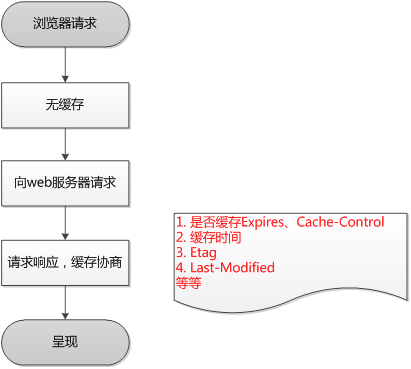
\includegraphics[width=0.8\textwidth]{./images/firstRequest.png}  
\end{figure}

下一次请求

\begin{figure}[!ht]
    \centering    
     \caption{\label{Fig:async} Asynchronous I/O model}
    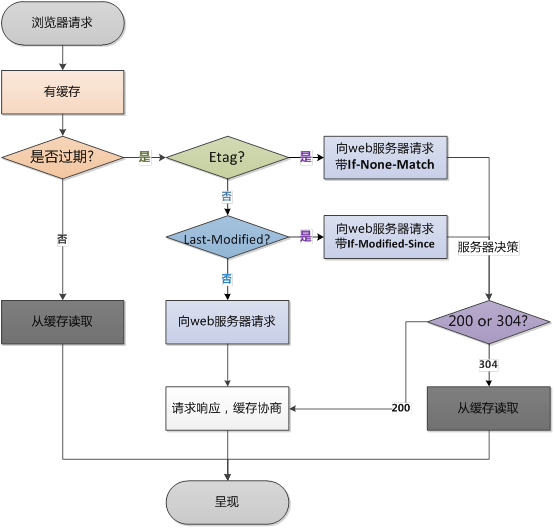
\includegraphics[width=0.8\textwidth]{./images/nextRequest.png}  
\end{figure}

\subsection{强缓存}

运维了解到此基础就OK, 需要了解更深可以查看网上资源

https://www.zhihu.com/question/20790576

https://www.cnblogs.com/wonyun/p/5524617.html
